\section{Event Detection Framework}
\label{sec:design:eventDetectionFramework}
The byte codes generated by the compiler can be further divided into three parts: event meta data, event filters and event matcher. Event meta data contains the description of the event types such as event type ID, event size and the individual attributes for each event. Event filters are the constraints defined for each event type. Event matcher schedules the execution for event detection according to the subscription and event relations.

\subsection{The Runtime Environment}
The runtime environment on each sensor node is similar to the VM-based approach \cite{mate} in the sense that the subscriptions are broken down into some basic operations. Such design choice is for the extensibility of the middleware so that different event detection mechanisms may be easily implemented through the operations. In addition to the VM-based runtime environment, as shown in Figure \ref{fig:pswarevm}, each sensor node has an event buffer where the detected events may be stored for composite event detection.

\begin{figure}
\centering
\figurecurrentwidth{pswarevm}
\caption{PSWare runtime environment}
\label{fig:pswarevm}
\end{figure}

The essential operations for our event detection framework is shown in Figure \ref{fig:eventdetectionframework2}. In this framework, the event matcher will first fetch the events from the event buffer and then evaluate them against the corresponding filters. If the event has been detected, then it will be transmitted over the network. Formally, the procedure of the event matcher can be shown in Procedure \ref{algo:eventMatcher} with some notations defined as:
\begin{itemize}
\item Event types: \(E=\{e_1, e_2 \cdots \}\)
\item For each \(e_n\in E\), its filter is: \(e_n\rightarrow filter\)
\item For each \(e_n\in E\), it has a set of events \(E_n=\{e_n^1, e_n^2 \cdots \}\) stored in the buffer.
\end{itemize}

\begin{figure}
\centering
\figurecurrentwidth{eventdetectionframework2}
\caption{Event detection framework}
\label{fig:eventdetectionframework2}
\end{figure}

\begin{algorithm}
\begin{algorithmic}[1]
\REQUIRE \(E\)
	\FORALL {\(e_n\in E\)}
		\FORALL {\(e_n^i\in E_n\)}
			\IF {\(e_n\) is primitive}
				\STATE result = evaluate\_primitive (\(e_n^i\))
				\IF {result == True}
					\IF {\(e_n\) is subscribed}
						\STATE deliver(\(e_n^i\))
					\ELSE
						\STATE forward(\(e_n^i\))
					\ENDIF
				\ENDIF
			\ELSE
				\FORALL {subevents \(e_m\) for \(e_n\)}
					\STATE evaluate\_composite(\(e_n^i\), \(e_m\), \(\cdots \))
				\ENDFOR
			\ENDIF
		\ENDFOR
	\ENDFOR
\end{algorithmic}
\caption{Procedure of the event matcher}
\label{algo:eventMatcher}
\end{algorithm}

There are several keys in the procedure. First, when the event matcher picks up the events of type \(e_n\) from the event buffer, it may use application specific mechanisms to pick up the desired events instead of trying all the possible combinations. Second, the 'deliver()' and the 'forward()' function are used to deliver the subscribed events or forward the events so that composite events may be detected. These two functions may also be application dependent to achieve high energy efficiency.

Figure \ref{fig:psware-interaction-simple} illustrates how different components in the middleware system interact with each other.

\begin{figure*}
\centering
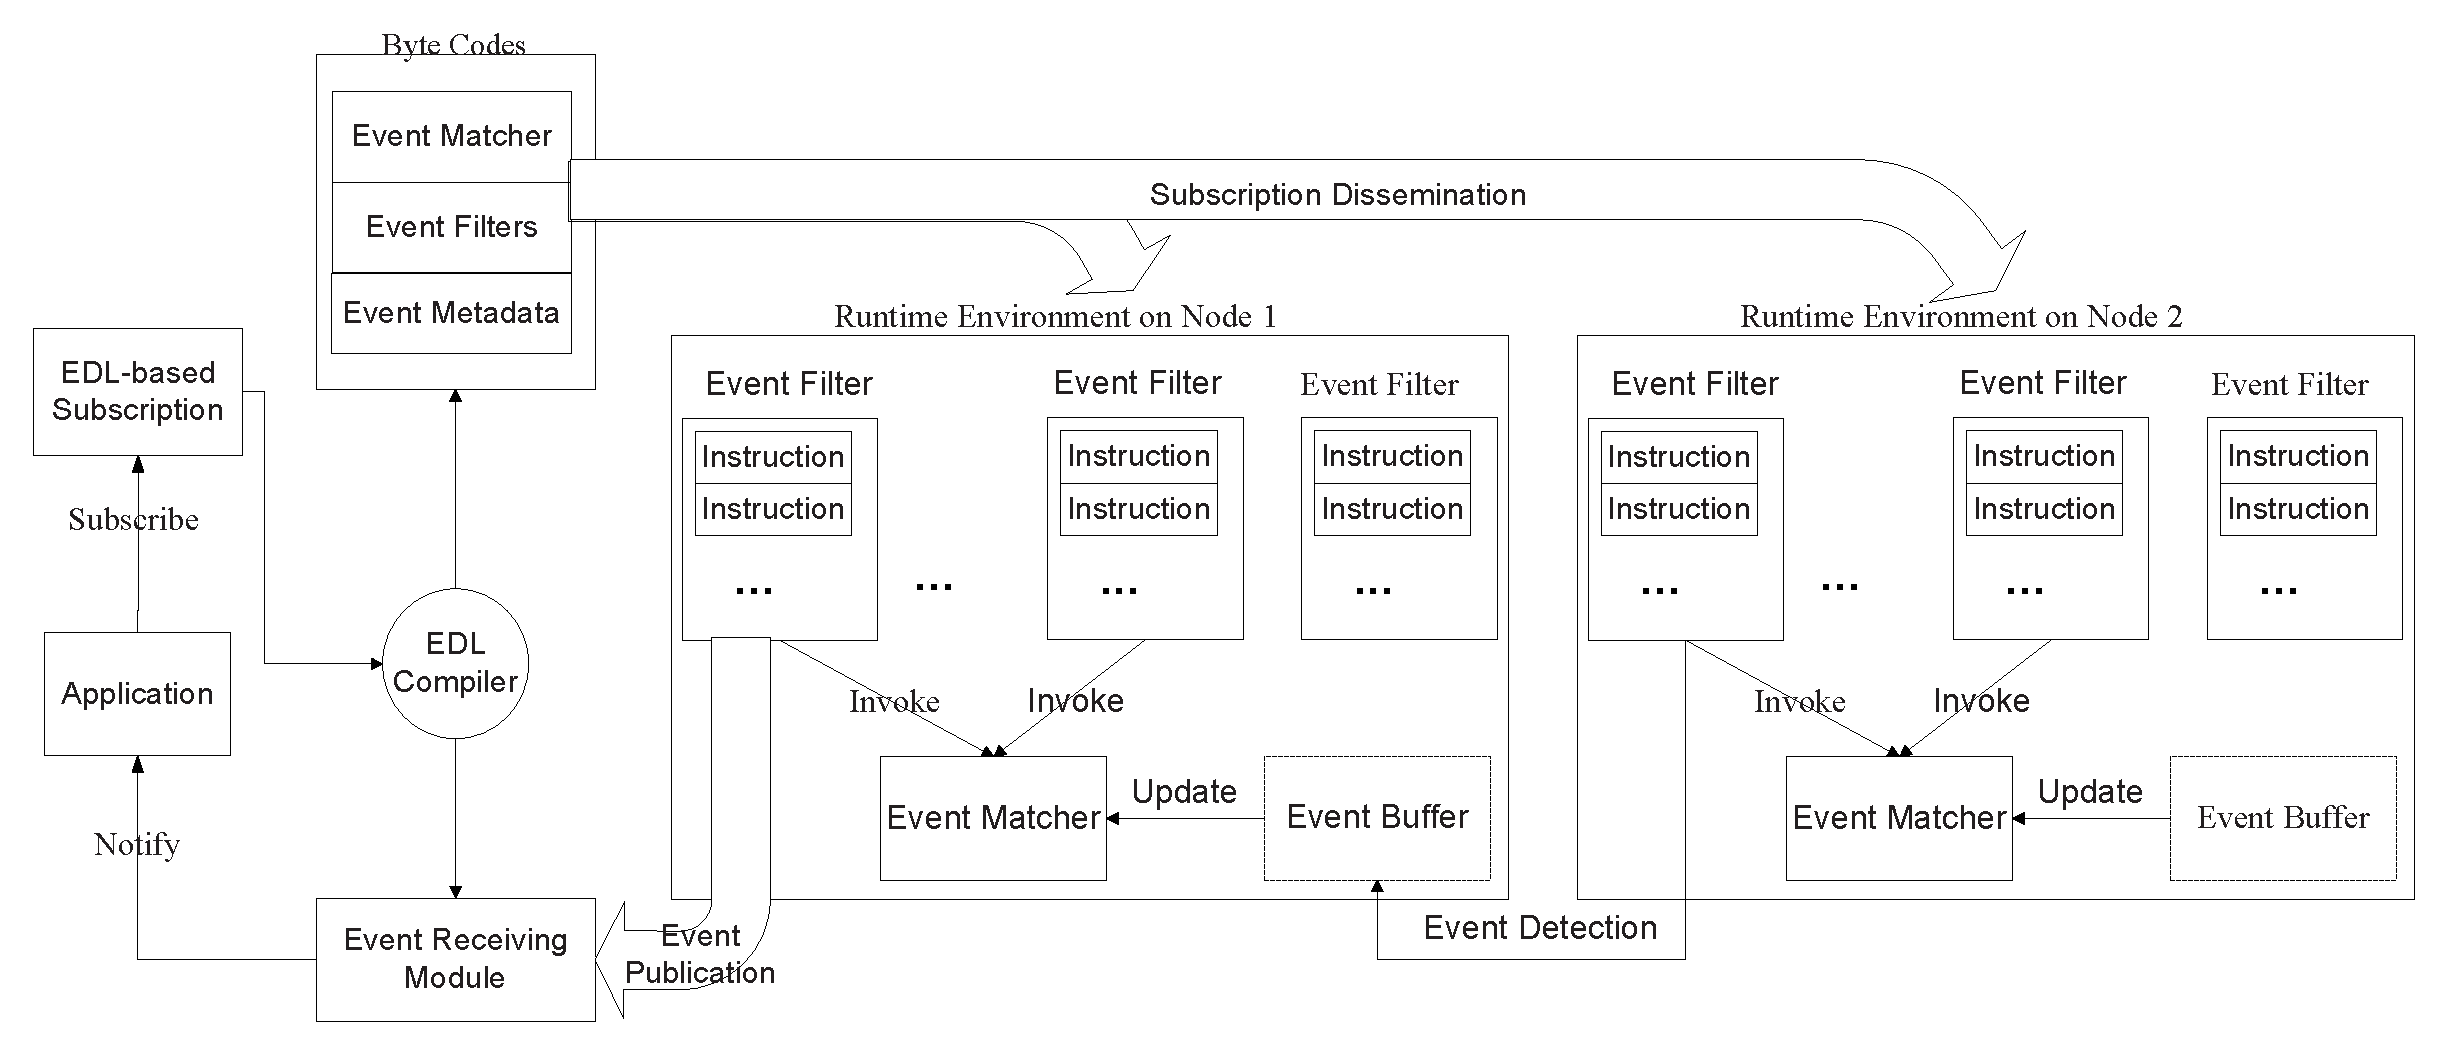
\includegraphics[width=\textwidth]{psware-interaction-simple}
\caption{PSWare components interaction}
\label{fig:psware-interaction-simple}
\end{figure*}
\subsection{Basic Instructions}
The design of our event detection framework makes it very suitable to be implemented using a VM-based architecture and this is how we implemented it in the bytecodes for the sensor nodes. Our VM-based runtime environment is based on Mat\'{e} \cite{mate}. It uses stack-based instructions which allow compact code size. We choose a VM-based runtime environment because it is more flexible in terms of interfacing with the EDL compiler and introducing new modules. Apart from the existing instructions which are already available in Mat\'{e}, we have mainly added the following instructions used specifically for event detection.
\begin{itemize}
	\item \emph{OPref}: whenever an event \(e\) is being evaluated, this instruction is invoked to obtain an instance of such event.
	\item \emph{OPoffset}: this instruction is involved right after the 'ref' instruction, in order to access individual attributes of the event instance.
	\item \emph{OPset}: if the attributes of an event need to be changed, this instruction will be used.
	\item \emph{OPget}: the 'get' instruction does the opposite of 'set' instruction. It will simply retrieve content of a specific attribute in an event.
	\item \emph{OPcreate}: is used to create a new instance of an event.
	\item \emph{OPeval}: is used to determine if an event happens or not.
\end{itemize}
For a complete list of all the instructions, please refer to Appendix \ref{appendix:isa} We give a simple example how EDL can be translated to the lower level runtime instruction sets. Consider a very simple event shown in Listing \ref{lst:originaledl}. The event will occur when the temperature reading on sensor node 5 is above 30. It's corresponding program for the VM is shown in Listing \ref{lst:translatededl}. Since 'SimpleEvent' is a primitive event, so every time it is being detected, a new instance of the event will be created. The ID of 'SimpleEvent' is \(1\). Here we also have another event called 'System' which is a built-in event provided by EDL as a place where all the sensor data can be obtained. The 'System' event has a default ID of \(0\) as shown on Line \ref{line:systemevent} in Listing \ref{lst:translatededl}. Each attributes in the event will have it's unique ID. In the example, the ID of the attribute is calculated simply by the order of their appearance. For example, temperature has the ID of \(0\) on Line \ref{line:systemevent}.

\begin{lstlisting}[caption=Original EDL program, label=lst:originaledl]
Event SimpleEvent {
	int temp=System.temp;
	int id=System.id;
} where {
	temp > 30 and
	id == 5
}
\end{lstlisting}
\begin{lstlisting}[caption=Translated EDL program, label=lst:translatededl]
alloc 1
ref 0 (*\label{line:systemevent}*)
offset 0
ref 1
offset 0
set
ref 0
offset 1
ref 1
offset 1 (*\label{line:idattr}*)
set
ref 1
offset 1
get
push 30
gt
ref 1
offset 1
get
push 5
eq
and
eval
\end{lstlisting}

\subsection{Customizing PSWare}
The event detection framework of PSWare is developed using NesC. As discussed in the previous section, many of the operations in PSWare can be defined according to applications. In this section, we describe how we can customize PSWare.

The first step is to implement a special module which acts like a device driver for PSWare. This module defines the sampling rate and a primitive event called 'System'. All the fields of other events are obtained from 'System'. The module needs to implement three interfaces: StdControl, SystemClock and SystemEvent as shown in Listing \ref{lst:systemEvent}. StdControl is a module for initialization purpose. SystemClock defines the sampling frequency. SystemEvent is used to obtain the pointer to the 'System' event.

\begin{lstlisting}[caption=API of the 'System' event, label=lst:systemEvent]
module SystemEventM {
	provides {
		interface StdControl;
		interface SystemEvent;
		interface SystemClock;
	}
}
interface SystemEvent {
	command EventInstanceInfo * get();
}
\end{lstlisting}

Once the 'System' event is defined, the application developers can further define their own functions for event delivery and event forwarding. We will show some examples in the next section. In addition, they can make use of the API provided by PSWare as shown in Listing \ref{lst:pswareAPI}.

\begin{lstlisting}[caption=API provided by PSWare, label=lst:pswareAPI]
interface EventMeta {
	command EventMetaInfo * getEventMeta(uint8_t subID);
	command bool isSubscribed(uint8_t subID);
	command bool isComposite(uint8_t subID);
	command bool isAggregate(uint8_t subID);
}
interface EventInstance {
	command EventInstanceInfo * createEvent(uint8_t subID);
	command int instanceAmount(uint8_t subID);
	command void deleteEvent(uint8_t subID, uint8_t instanceID);
	command EventInstanceInfo * getEventInstance(uint8_t subID, int idx);
}
interface EventMatcher {
	command bool selectSubevent(EventInstanceInfo * composite, EventInstanceInfo * subevent);
	command result_t eventDetected(uint8_t subID, uint8_t instanceID, bool detectionResult);
	command result_t eventDelivery(uint8_t subID, uint8_t instanceID, bool detectionResult);
}
\end{lstlisting}

These API provides the necessary functionalities for accessing modules such as event meta data or the event buffer (as in EventInstance). To implement application specific event detection mechanisms, application developers simply need to override the commands provided in the EventMatcher interface. The 'selectSubevent()' command is used to determine if a sub-event (in the parameter subevent) should be used to detect a composite event (in the parameter composite).